\subsection{Deployments}

Como foi explicado anteriormente, um dos requisitos definidos  era a criação de um ambiente de \textit{CI/CD} que permitisse simplificar o processo de desenvolvimento, facilitando a disponibilização de novas versões.

A plataforma Azure disponibiliza a funcionalidade \textit{Pipelines}. Com o recurso à linguagem YAML, esta permite definir os trabalhos que os "agentes" definidos pelo utilizador

Finalmente, utilizando a ferramenta Docker é possível "empacotar" o código numa só unidade que funciona de forma igual em diferentes máquinas. Esta funcionalidade será feita numa máquina Linux Ubuntu 24.04.2. 

\subsubsection{Definição dos agentes}

No contexto do Azure Pipelines um agente (em inglês, \textit{Agent}) é a máquina indica ao Azure Pipelines que executará os trabalhos pedidos, como, por exemplo, compilar o projeto. 

Neste caso iremos indicar ao Azure Pipelines para que utilize a nossa máquina como um agente. O agente irá executar dentro de um \textit{container Docker}.

A Microsoft oferece ferramentas para ajudar neste processo \cite{run-a-self-hosted-agent-in-docker}. O script que estabelece a relação entre os agentes e os serviços Azure, tal como o ficheiro \textit{.Dockerfile} necessário para a construção da Imagem Docker poderá ser encontrado nos anexos \ref{app:pipeline-start.sh} e \ref{app:dockerfile-pipeline-agent} respetivamente.

Após a criação do agente basta iniciar o \textit{container Docker}, tendo em atenção à indicação das variáveis de ambiente necessárias. A figura \ref{fig:start-docker-agent} demonstra isso mesmo, com censura a qualquer informação sensivel à organização.

\begin{figure}[h!tbp]
    

\begin{lstlisting}
    sudo docker run -d 
        -e AZP_URL="https://dev.azure.com/blended4future2025" 
        -e AZP_TOKEN="******" 
        -e AZP_POOL="*******" 
        -e AZP_AGENT_NAME="*****" 
        --name "azp-agent-linux" 
        devops-agent:linux
\end{lstlisting}


\caption{Script de inicialização do Container Docker para o agente do Azure Pipelines}
\label{fig:start-docker-agent}

\end{figure}

Logo após, é possivél ver o agente disponível no Azure DevOps (Figura \ref{fig:agent-devops}). 

\begin{figure}[h!tbp]
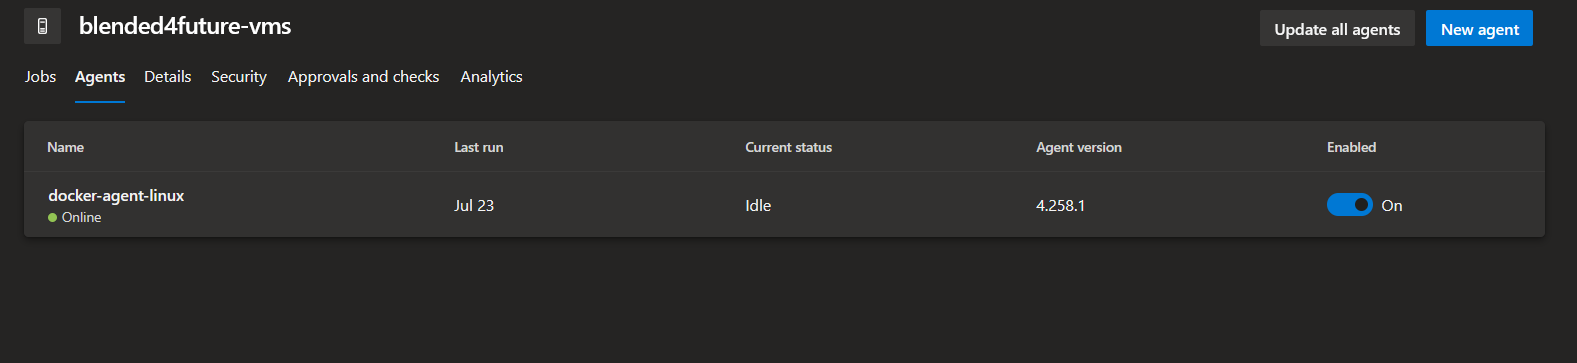
\includegraphics[width=\linewidth]{capitulos/cap4-implementacao/assets/devops-agent.png}
\caption{Agente disponbilizado no Azure DevOps}
\label{fig:agent-devops}
\end{figure}

\subsubsection{Trabalhos da pipeline}

O conceito de trabalho (em inglês, \textit{Job}) é de extrema importância no Azure Pipelines. Este permite definir ações e os seus respetivos passos para atingir um objetivo.

Nesta secção demonstra-se a \textit{pipeline} criada e os respetivos passos por ela tomados, utilizando como exemplo a definida para o módulo \textit{frontend}. A versão completa deste ficheiro poderá ser encontrada no apêndice \ref{app:pipeline-yaml}. 

\begin{figure}[h!tbp]
    \centering
    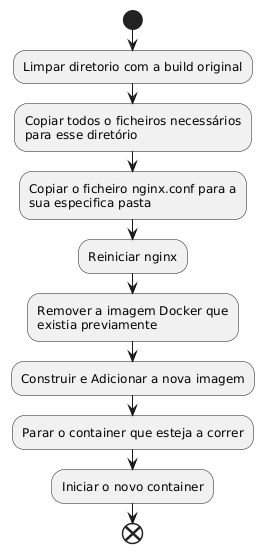
\includegraphics[width=0.3\linewidth]{capitulos/cap4-implementacao/assets/pipeline-activity-diagram.png}
    \caption{Diagrama de atividade representante da Pipeline de construção de uma nova versão}
    \label{fig:pipeline-ad}
\end{figure}


Na figura \ref{fig:pipeline-ad}, é possível ver o um diagrama de atividade que descreve cada passo feito por este trabalho.

\begin{lstlisting}[caption={Trigger - Pipeline},label={lst:pipeline-trigger}]
trigger:
    branches:
        include:
            - main
\end{lstlisting}


A listagem \ref{lst:pipeline-trigger}, descreve o gatilho (em inglês, \textit{trigger}) de ativação da pipeline. Neste caso qualquer \textit{commit} no \textit{branch} "main" irá ativar os trabalhos definidos.

É importante enaltecer que existem variáveis que foram definidas externamente através do Azure DevOps e que são utilizadas ao longo da pipeline. Estas são:

\begin{itemize}
    \item \textbf{CONTAINERNAME}: Nome que o \gls{Container} terá quando for criado.
    \item \textbf{FRONTENDBUILDPATH}: Caminho para o qual o projeto será copiado para.
    \item \textbf{VMBUILDPATH}: Caminho para o qual a \gls{Build} do projeto irá ser colada em.
\end{itemize}

Finalmente, cada passo segue o conceito apresentado na figura \ref{fig:pipeline-ad}. Especial atenção para o uso de \lstinline|SSH@0|\cite{docs-SSH0}, esta é uma \textit{task} pre disponibilizada para estabelecer uma conexão SSH a uma máquina alvo. A chave está definida como segredo e é importado no início do ficheiro quando ocorre uma referência ao grupo de variáveis "ssh".
